%%%%%%%%%%%%%%%%%%%%%%%%%%%%%%%%%%%%%%%%%%%%%%%%%%%%%%%%%%%%
%%% LaPreprint: PREPRINT TEMPLATE
%%%%%%%%%%%%%%%%%%%%%%%%%%%%%%%%%%%%%%%%%%%%%%%%%%%%%%%%%%%%

% Here I could talk about what one should do in this document.
% Instead I'll refer you to the explore on your own as check the Github Repo. :-)
% Line spacing is 1.2 by default (can't be smaller).

%%%%%%%%%%%%%%%%%%%%%%%%%%%%%%%%%%%%%%%%%%%%%%%%%%%%%%%%%%%%
%%% PREAMBLE
%%%%%%%%%%%%%%%%%%%%%%%%%%%%%%%%%%%%%%%%%%%%%%%%%%%%%%%%%%%%

% Declare document class
\documentclass[9pt,biorxiv,lineno]{preprint}
% Choose between "biorxiv", "medrxiv", "arxiv" and "chemrxiv". Otherwise defaults to Preprint.
% Use the "onehalfspacing" option for 1.5 line spacing
% Use the "doublespacing" option for 2.0 line spacing
% Use the "lineno" option for line numbers
% Use the "endfloat" option to place floats after the bibliography

% Import packages
\usepackage{lipsum}     % Required to insert dummy text
\usepackage[version=4]{mhchem} % For chemical notation
\usepackage{siunitx}    % For SI units
\usepackage{pdflscape}  % For putting pages in landscape mode
\usepackage{rotating}   % For rotating specific elements
\usepackage{textgreek}  % Greek symbols
\usepackage{gensymb}    % Symbols
\usepackage[misc]{ifsym} % For the \Letter symbol
\usepackage{orcidlink}  % For the \orcidlink
\usepackage{listings}   % For inserting code chunks
\usepackage{colortbl}   % For Knitr table colouring
\usepackage{tabularx}   % For making Knitr tables compatible
\usepackage{longtable}  % For multi-page tables
\usepackage{subcaption}
\usepackage{multirow}
\usepackage{snotez}     % For sidenote environments. enotez for endnotes

% Make declarations
\DeclareSIUnit\Molar{M}

% Please note that these options may affect formatting.

%%%%%%%%%%%%%%%%%%%%%%%%%%%%%%%%%%%%%%%%%%%%%%%%%%%%%%%%%%%%
%%% ARTICLE SETUP
%%%%%%%%%%%%%%%%%%%%%%%%%%%%%%%%%%%%%%%%%%%%%%%%%%%%%%%%%%%%

% Paper title
\title{LaPreprint: \\ A Preprint Template for \LaTeX}

% Authors - you can use \orcidlink{} and \authfn{} - see contribution note
\author[ \orcidlink{0000-0002-9998-0058} 1 \Letter]{Mikkel Roald-Arb\o l}
\author[2]{Co-author}

% Affiliations
\affil[1]{School of Life Sciences, University of Sussex}
\affil[2]{University of Somewhere}

% Correspondence
\correspondence{https://github.com/roaldarbol/LaPreprint/issues}{MRA}

% Contribution note
\contribution[\authfn{1}\authfn{2}\authfn{3}]{Here's a few symbols to denote contribution specifics, e.g. authors who contributed equally to the work.}

% Present address of corresponding author
\presentaddress[]{Evolution, Behaviour and Environment, School of Life Sciences, University of Sussex, Biology Road, Brighton, BN1 9RH, United Kingdom}

% Data availability statement, funding and competing interests.
\data[]{Data availability statement. Preprocessed data could be available e.g. on \href{https://zenodo.org/}{Zenodo}.}
\funding[]{MRA was supported by funding from the Leverhulme Foundation. The funders had no role in the template design or decision to publish.}
\compint[]{The author declare no competing interests.}


% Surname of the lead author(s) for the running footer
\leadauthor{Roald-Arb\o l}
\shorttitle{A Preprint Template for \LaTeX}

%%%%%%%%%%%%%%%%%%%%%%%%%%%%%%%%%%%%%%%%%%%%%%%%%%%%%%%%%%%%
%%% ARTICLE START
%%%%%%%%%%%%%%%%%%%%%%%%%%%%%%%%%%%%%%%%%%%%%%%%%%%%%%%%%%%%

\begin{document}
\maketitle
\begin{abstract}
\lipsum[1]
\end{abstract}
\section{Introduction} \label{intro}
Let's begin with some great papers for those interested in radically improving the scientific infrastructure \citep{Pooley2021, Bezuidenhout2021,Brembs2021}.
\lipsum[1-2]
\lipsum[3-4]
\sidenote{This is a sidenote made with the \textbackslash sidenote package. \lipsum[1]}
\section{Methods \& Materials} \label{methods}
\subsection{Tagging \& pinning}
Ants were selected from their nests based on their relatively large size and high activity. Before being placed in the set-up described below, each individual ant was marked with a distinct pattern of coloured paint spots (Humbrol Enamel, Hornby Hobbies Ltd, Kent, UK) on its thorax and abdomen for posterior identification. Tagged ants were left in a box with inside walls covered in fluon (ASC 109, Blades Biological Ltd, Edenbridge, UK) for at least 30 minutes before pinning for the paint to dry. Ants were then anaesthetized with ice and placed under a microscope (210444, Olympus Corporation, Tokyo, Japan). A fine minutien pin (0.1 mm diameter, 1 cm length; Fine Science Tools GmbH, Heidelberg, Germany), with the top third bent around 45$\degree$ was attached to the most posterior segment of their thorax using fast dry UV glue (5SF-MC12/6, 5 Second Fix). Painted and pinned ants were left inside the same fluoned box until being restrained in the virtual reality set-up.
\sidenote{\lipsum[1]}
\sidenote{\lipsum[1]}
\sidenote{\lipsum[1]}

\subsection{Virtual reality setup}
In short, our virtual reality (VR) system consisted on a walking platform which movement was recorded and in turn changed the coordinates of the projected virtual world accordingly. This created a closed-loop between the ants’ movement and the visual stimuli, allowing them to navigate in a virtual environment (figure \ref{fig:setup}).

To reduce the presence of visual cues between the ant and the projection, a 3D printed custom made floor was placed above the polystyrene ball, with a 2 cm diameter hole in the centre where the ant was placed (figure \ref{fig:setup}).

\begin{figure}
\centering
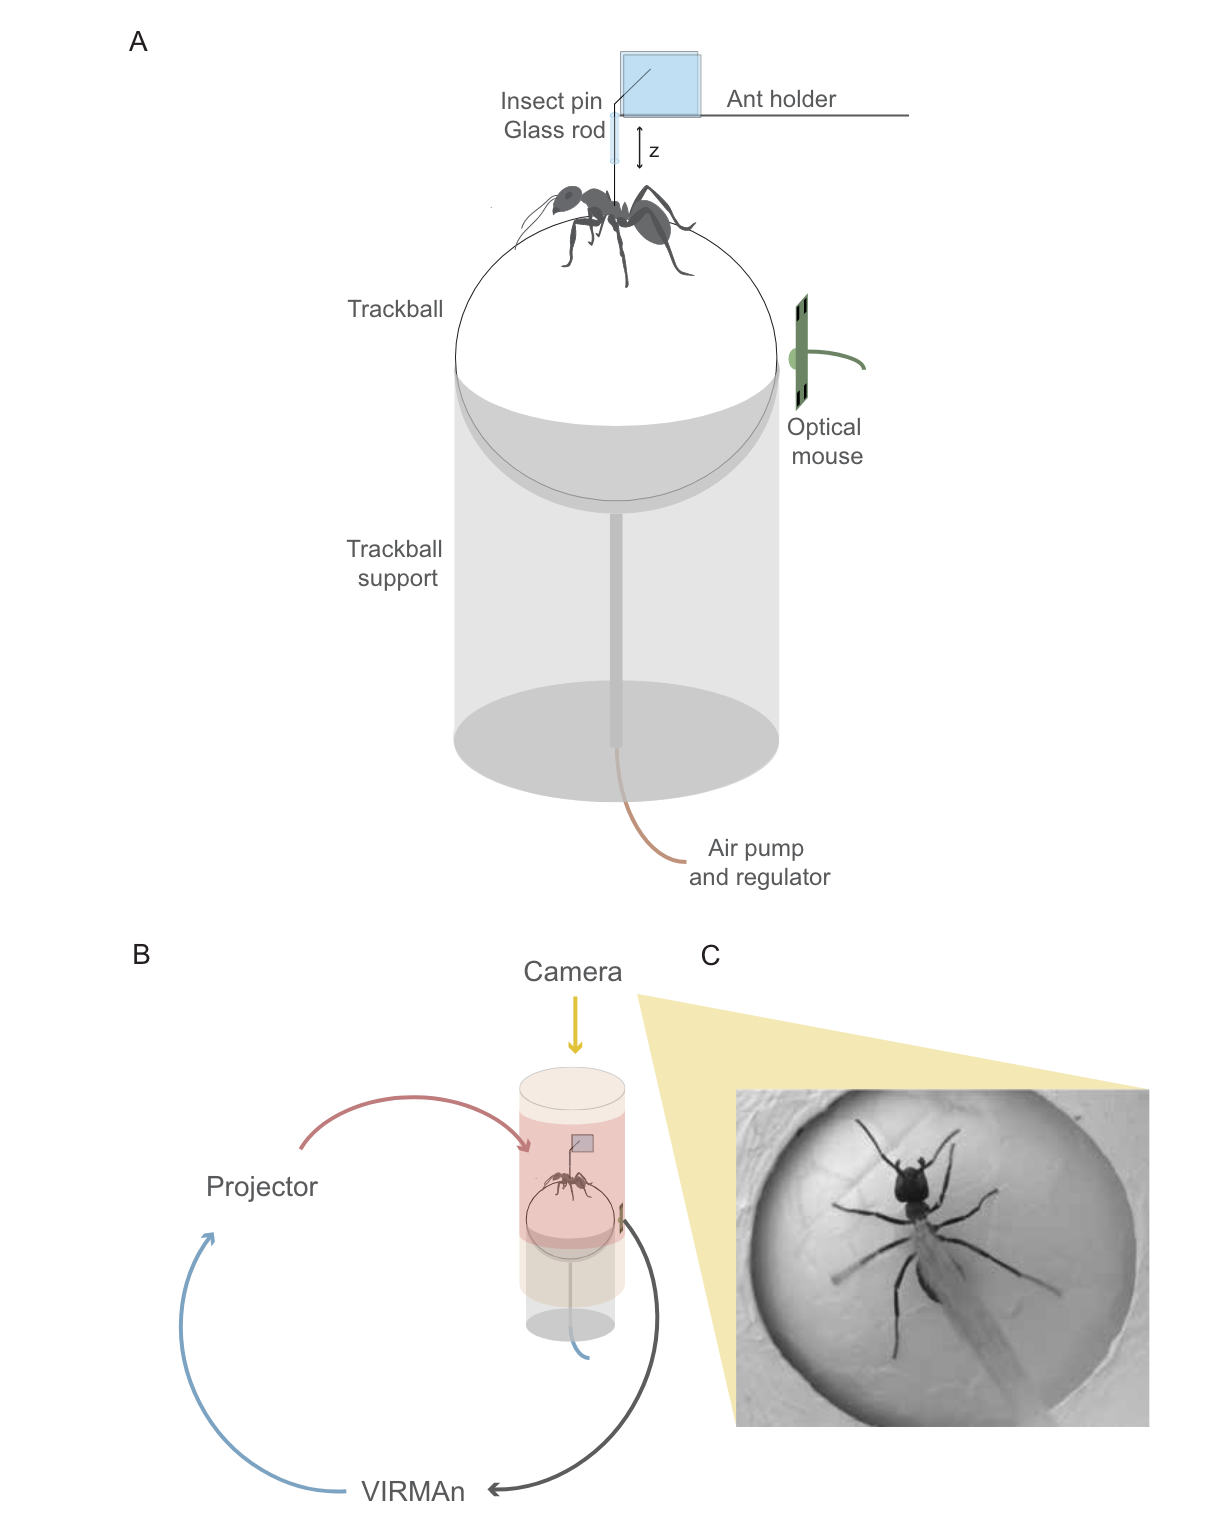
\includegraphics[width=\hsize]{figures/setup.png}
\caption{\textbf{Schematic diagram of the virtual reality paradigm}. A) Wood ants are placed on top of a polystyrene ball (trackball), seating on a metallic cup (trackball support) perforated inside to allow pressure regulated air flow from an air pump to support the trackball. The ant is restrained by an insect pin glued to the posterior portion of the thorax. The insect pin is kept in place by a glass rod and two custom made plastic structures that allow the ant to move up and down (z) but not rotate on top of the ball. As the ant walks, the air supported trackball moves underneath, which is recorded by an optical mouse. B) The optical mouse is connected to a computer running the Matlab package VIRMEn. VIRMEn creates a virtual world and changes it according to the optical mouse recordings. The virtual world is displayed to the ant through a projector connected to the same computer onto a tracing paper cylinder surrounding the ant, trackball and support. C) A camera placed above the set-up records the ant at all times. A portion of the trackball is covered by a custom made white floor to reduce the presence of visual cues between the ant and the virtual world.
}
\label{fig:setup}
\end{figure}




\section{Results} \label{results}
\lipsum[1-4]
\section{Discussion} \label{discussion}
\lipsum[1-3]
\subsection{Acknowledgment}
Insert the Acknowledgment text here.

\subsection{Author contributions}
Maybe with a contribution table instead...
Conceptualization: E.S., B.H.; Methodology: B.H.; Software: B.H.; Validation: S.R.; Formal analysis: S.R.; Investigation: E.S.; Resources: B.H.; Writing - original draft: E.S.; Writing - review \& editing: S.R., B.H.; Visualization: S.R.; Supervision: B.H.; Project administration: B.H.; Funding acquisition: B.H.
% According to https://journals.biologists.com/jeb/pages/author-contributions

\subsection{Supplementary}
Insert the supplementary text text here.
\bibliography{bibliography}

% DON'T EDIT. If "endfloat" option is enabled all floats appear before appendices
\if@endfloat\clearpage\processdelayedfloats\clearpage\fi 


%%%%%%%%%%%%%%%%%%%%%%%%%%%%%%%%%%%%%%%%%%%%%%%%%%%%%%%%%%%%
%%% SUPPLEMENTARY MATERIAL / APPENDICES
%%%%%%%%%%%%%%%%%%%%%%%%%%%%%%%%%%%%%%%%%%%%%%%%%%%%%%%%%%%%

\begin{appendix}
\begin{appendixbox}\label{app:ttt}
    \begin{appendixbox}
\label{app:ttt}
\section{TTT, by Piet Hein}
Problems worthy \\
of attack \\
prove their worth \\
by hitting back. \\
\\
Put up in a place \\
where it's easy to see \\
the cryptic admonishment\\
    T.T.T. \\
\\
When you feel how depressingly \\
slowly you climb, \\
it's well to remember that\\
Things Take Time. \\
\\
The road to wisdom? - Well, it's plain\\
and simple to express: \\
   Err \\
   and err \\
   and err again \\ 
   but less \\
   and less \\
   and less. \\

\end{appendixbox}

\end{appendixbox}
\begin{appendixbox}
    \section{Key resources}
Here could be a nice table. Instead you get more Latin text. \newline
\lipsum[1-2]

% Make your own table style https://tex.stackexchange.com/questions/94799/how-do-i-color-table-columns
\end{appendixbox}
\end{appendix}


%%%%%%%%%%%%%%%%%%%%%%%%%%%%%%%%%%%%%%%%%%%%%%%%%%%%%%%%%%%%
%%% ARTICLE END
%%%%%%%%%%%%%%%%%%%%%%%%%%%%%%%%%%%%%%%%%%%%%%%%%%%%%%%%%%%%

\end{document}
